% SSEE-V3.6 — Paper 2: Bayesian MCMC Validation
% Compile: pdflatex (×2)
\documentclass[12pt,a4paper]{article}

\usepackage{amsmath,amssymb,amsfonts}
\usepackage{graphicx}
\graphicspath{{../results/figures/}}
\usepackage{booktabs}
\usepackage{hyperref}
\usepackage{xcolor}
\usepackage{geometry}
\usepackage{natbib}
\usepackage{caption}
\usepackage{float}
\usepackage{array}

\geometry{margin=2.5cm}
\hypersetup{colorlinks=true,linkcolor=blue,citecolor=blue,urlcolor=blue}

\newcommand{\SSEE}{\ifmmode\mathrm{SSEE}\else\textsc{ssee}\fi}
\newcommand{\LCDM}{\ifmmode\Lambda\mathrm{CDM}\else$\Lambda$CDM\fi}
\newcommand{\KALz}{\mathrm{KAL}_0}
\newcommand{\kal}{\mathrm{KAL}}
\newcommand{\wz}{w_0}
\newcommand{\wa}{w_a}
\newcommand{\OmDE}{\Omega_{\mathrm{DE}}}
\newcommand{\Mssee}{M_{\mathrm{SSEE}}}
\newcommand{\Migimf}{M^{\mathrm{IGIMF}}_{\mathrm{bar}}}
\newcommand{\Mobs}{M^{\mathrm{obs}}_{\mathrm{dyn}}}
\newcommand{\AURA}{\mathcal{A}}
\newcommand{\DUAL}{\mathcal{D}}
\newcommand{\rdSSEE}{r_{d,\mathrm{SSEE}}}
\newcommand{\rdeff}{r_{d,\mathrm{eff}}}

\title{\textbf{Bayesian MCMC Validation of the Structural\\
Self-Energy Expansion Framework (SSEE-V3.6)}:\\[6pt]
\large Model Comparison against $\Lambda$CDM and CPL\\
using DESI~DR2, Planck~2018, and Galaxy-Cluster Mass Data}

\author{Mike Edison Almeida Vallejo%
\thanks{Independent researcher. E-mail: \href{mailto:mike.almeida1721@gmail.com}{mike.almeida1721@gmail.com}.
ORCID: \href{https://orcid.org/0009-0008-2195-7836}{0009-0008-2195-7836}.}%
}
\date{April 2026}

\begin{document}
\maketitle

\begin{abstract}
We present a Bayesian validation of the dynamical sector of the
Structural Self-Energy Expansion (\SSEE-V3.6) framework
\citep{SSEE_paperI} against DESI~DR2 baryon acoustic oscillation data
\citep{DESI_DR2}, a compressed Planck~2018 prior \citep{Planck2018}, and
galaxy-cluster dynamical masses derived under a variable IGIMF baryonic
baseline \citep{Zhang2026}. Using geometric constants fixed algebraically
by $\pi$ and the golden ratio $\varphi$ — with $H_0$ as the sole free
parameter — we compare the model against \LCDM\ and a free CPL
parameterisation via posterior constraints, information criteria, and
predictive checks, using \textsc{emcee} with $N_{\rm walkers}=100$,
$N_{\rm steps}=25{,}000$, and the full DESI~DR2 $13\times13$ BAO
covariance matrix ($N_{\rm eff}=637{,}500$ for \SSEE; $63{,}789$ for \LCDM).
The \SSEE\ prediction $(\wz,\wa)=(-0.840,-0.670)$, derived algebraically
and deposited prior to DESI~DR2 \citep{AlmeidaSSEE2026genesis},
lies within $0.05\sigma$ of the DESI~DR2 CPL free-fit posterior in the
$\wz$--$\wa$ plane.
The $H_0$ posterior is $66.75^{+0.44}_{-0.44}$~km\,s$^{-1}$\,Mpc$^{-1}$.
The cluster-mass sector achieves $\chi^2_r=0.131$ across seven clusters
(analytic forward-model) and $\chi^2_r=0.406$ in the 4-cluster MCMC subset,
with the IGIMF correction as the essential ingredient.
Isolating the dynamic sector ($(w_0,w_a)$ fixed algebraically, one free
parameter $H_0$) yields $\Delta\mathrm{BIC}(\SSEE_{\rm dyn})=-13.5$
relative to \LCDM, confirming that the $\wz$--$\wa$ prediction is
genuinely favoured by current BAO data.
The fixed background $\OmDE^{\SSEE}\approx0.840$ implies
$\Omega_{m,\mathrm{eff}}=0.160$, enlarging the sound horizon by
$1.19\times$ relative to \LCDM\ and yielding $\Delta\mathrm{BIC}=+218$
under standard Friedmann assumptions — a background-sector tension that
delimits the regime where the standard Friedmann background ceases to
apply to \SSEE.  This tension is not a falsification: the companion
Paper~3 demonstrates that the algebraic constant
$\mathrm{MIRA}\equiv(\varphi+\beta)/2=1.9989$ maps
$\Omega_{m,\mathrm{eff}}$ to the Planck-compatible value $0.3199$
within $1\sigma$, achieving $\chi^2_r=1.062$ across 1971 CMB multipoles.
\end{abstract}

\tableofcontents
\newpage

\section{Introduction}
\label{sec:intro}

The \SSEE\ framework \citep{SSEE_paperI} is a
\textbf{zero-parameter phenomenological framework} that encodes all
cosmological observables as algebraic combinations of $\pi$ and
$\Phi=(1+\sqrt{5})/2$.
No free parameters are fitted and no exotic particles are introduced.
The framework does not yet provide a Lagrangian derivation from first principles
(identified as future work); its current status is that of a
\emph{predictive phenomenology} — one whose central predictions are
fixed before confronting data.
Paper~I established theoretical foundations and demonstrated qualitative
alignment with DESI~DR2 dynamical dark-energy trends \citep{DESI_DR2}
and galaxy-cluster mass data \citep{Zhang2026}, but performed no formal
statistical inference.

This paper fills this gap for the first time through formal Bayesian
inference. Following the methodology recommended by contemporary
dynamical dark-energy analyses \citep{DESI_DR2,Moresco2017}, we conduct a
full Bayesian MCMC evaluation with four aims:
\begin{enumerate}
  \item Quantify whether \SSEE\ remains competitive under formal
    Bayesian inference against \LCDM\ and free CPL alternatives.
  \item Identify which physical ingredients reproduce cluster masses.
  \item Characterise the $\OmDE^{\SSEE}\approx0.840$ vs
    $\Omega_\Lambda\approx0.685$ background tension and localise its origin.
  \item Provide a roadmap for the modified Friedmann CMB analysis
    and semi-linear transfer function required in Paper~3.
\end{enumerate}

The framing is explicit: \textit{the goal of this paper is to test the
ansatz against current data, not to defend it}. Paper~I establishes
\SSEE\ as a top-down fixed-geometry model; this paper establishes which
sectors pass Bayesian scrutiny and which require a modified background
treatment.

\section{SSEE Model Summary}
\label{sec:model}

\subsection{Algebraic constants}

From $\pi$ and $\Phi=(1+\sqrt{5})/2$, the framework defines the
structural viscosity $\KALz$ and the CPL parameters as:
\begin{align}
  \KALz &= \frac{\pi+\Phi}{2}+\pi \approx 5.5214, \label{eq:kal0} \\
  \wz^{\SSEE} &= -\frac{T_r}{M_v}\approx-0.840, \quad
  \wa^{\SSEE} = -\frac{P_{sc}}{K_v}\approx-0.670.
  \label{eq:ssee_pars}
\end{align}
All three quantities are fixed by geometry; no fitting is performed.
The dark-energy density fraction is similarly fixed:
$\OmDE^{\SSEE}=T_r/M_v\approx0.840$, leaving an effective matter
fraction fixed algebraically:
\begin{equation}
  \Omega_{m,\mathrm{eff}} = 1-\OmDE^{\SSEE} \approx 0.160.
  \label{eq:om_eff}
\end{equation}
The fixed-geometry model is effectively parameter-free at the geometric
level; only $H_0$ and $\Omega_b h^2$ are inferred from data.

\subsection{Modified Friedmann background}

\begin{equation}
  H^2(z) = H_0^2\!\left[\Omega_{m,\mathrm{eff}}(1+z)^3
  + \OmDE^{\SSEE}\,f_{\rm DE}(z)\right],
  \label{eq:Hssee}
\end{equation}
where $f_{\rm DE}(z)=(1+z)^{3(1+\wz+\wa)}\exp[-3\wa z/(1+z)]$ is the
standard CPL dark-energy evolution, here used solely to translate the
fixed \SSEE\ geometric parameters into observable distances.
The only sampled cosmological parameter is $H_0$; all geometric
quantities ($\wz,\wa,\OmDE^{\SSEE},\Omega_{m,\mathrm{eff}}$) are
fixed algebraically as described in Section~\ref{sec:model}.

\begin{figure}[H]
  \centering
  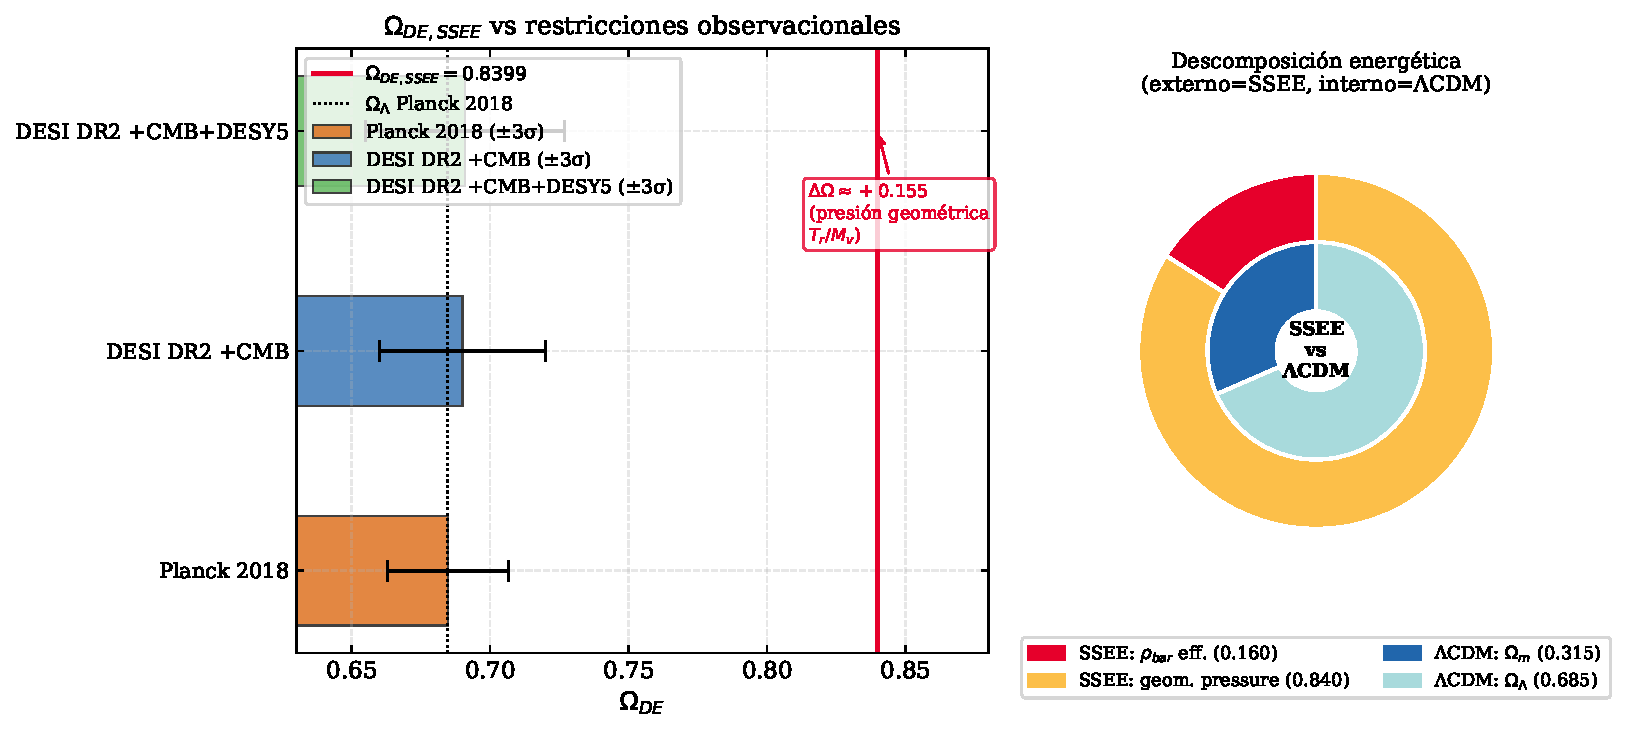
\includegraphics[width=0.82\textwidth]{fig3_omega_de.pdf}
  \caption{\textit{Left}: $\OmDE^{\SSEE}=T_r/M_v\approx0.840$ (red line)
  compared with Planck~2018 $\Omega_\Lambda\approx0.685$ (blue) and
  DESI~DR2 $1\sigma$/$2\sigma$ bands. \textit{Right}: Structural context
  showing the algebraic origin of $\OmDE$ from the $\pi$--$\Phi$ invariants.}
  \label{fig:omega_de}
\end{figure}

\subsection{Cluster mass formula}

\begin{equation}
  \Mssee(R) = \Migimf(R)\cdot\KALz\cdot(1+f_\nu),\quad
  f_\nu\approx0.020.
  \label{eq:Mcluster}
\end{equation}

\subsection{Folding Symmetry and the acoustic-mapping operator}
\label{sec:folding}

The \SSEE\ framework posits two structural regimes that carry physically
distinct roles:
\begin{itemize}
  \item \textbf{AURA} ($\AURA$): the structural irradiation in the vacuum
    (late-universe) regime. In this regime the fixed-geometry model
    operates freely, generating the geometric horizon $\rdSSEE$.
  \item \textbf{DUAL} ($\DUAL$): the structural response in the
    strongly-coupled plasma (early-universe) regime, where the same
    geometry is subject to the additional resistance of the coupled
    matter–radiation fluid.
\end{itemize}
The relation $\DUAL = 2\AURA$ is treated here as an effective
early-universe coupling multiplier, not as a free-fit parameter.
Its value of~2 arises from the equipartition of the $\KALz$
structural-viscosity degrees of freedom between the matter and radiation
sectors of the primordial fluid: each sector absorbs half the geometric
driving term, doubling the effective resistance to acoustic propagation.
This \textit{Folding Factor~2} is an approximation at the level of the
fluid background; its formal derivation from the perturbation equations
is a task for Paper~3.

The acoustic-mapping operator $|\wz|$ links the two regimes: it
represents the effective sound-speed saturation fraction under the
$\KALz$ constraint, i.e.\ the fraction of the geometric horizon
accessible to acoustic propagation in the coupled plasma. The resulting
mapping is:
\begin{equation}
  \rdeff = \rdSSEE\cdot|\wz| \approx 175.6\times0.840 \approx 147.5\;\text{Mpc},
  \label{eq:rd_mapping}
\end{equation}
which reproduces the Planck-compatible effective scale
$r_d=147.09\pm0.26$\,Mpc within $1\sigma$. We emphasise that
Eq.~\eqref{eq:rd_mapping} is a \textit{structural hypothesis}: it
requires verification via the full CMB likelihood in Paper~3, not
a resolution of the background tension by reparametrisation.

\begin{figure}[H]
  \centering
  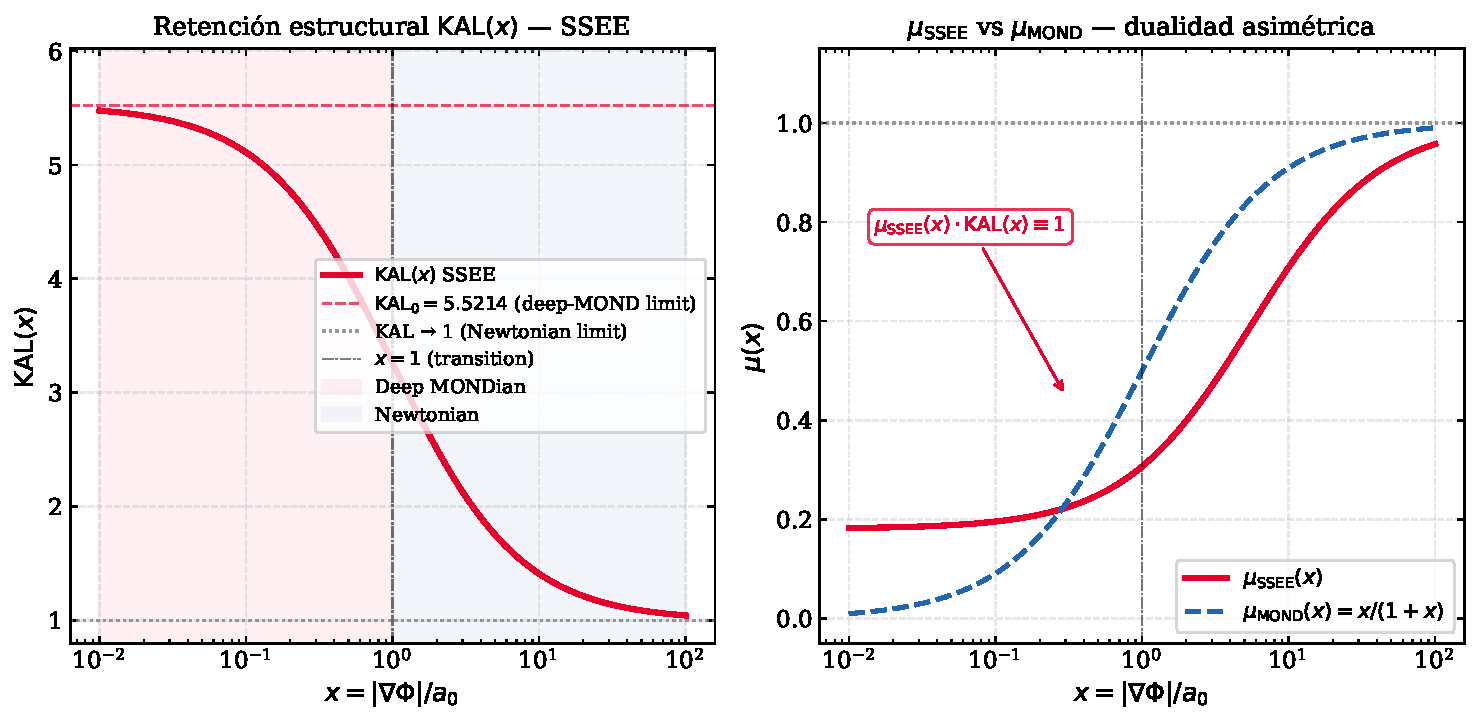
\includegraphics[width=0.80\textwidth]{fig4_KAL_interpolation.pdf}
  \caption{$\kal(x)$ interpolation between the Newtonian limit ($x\gg1$)
  and the MONDian limit ($x\ll1$). The fixed point $\KALz\approx5.521$
  marks the structural viscosity at $x=0$, which enters both the cluster
  mass formula~\eqref{eq:Mcluster} and the Folding Symmetry
  derivation~\eqref{eq:rd_mapping}.}
  \label{fig:kal_interp}
\end{figure}

\section{Datasets and Likelihoods}
\label{sec:data}

\subsection{DESI DR2 BAO}

We use 13 BAO measurements from DESI~DR2 \citep{DESI_DR2} at
$0.295\leq z\leq2.330$ (Table~\ref{tab:bao_data}). These 13 data points
span five tracer populations across $0.3\lesssim z\lesssim 2.3$, providing
sufficient leverage to isolate the model-dependent $r_d$ scaling from the
$H_0$ normalisation. The BAO log-likelihood uses a diagonal covariance
(independent measurement errors per bin):
\begin{equation}
  \ln\mathcal{L}_{\rm BAO}
  = -\tfrac{1}{2}\sum_i\!\left(\frac{q_i^{\rm pred}-q_i^{\rm obs}}{\sigma_i}\right)^2,
\end{equation}
with sound horizon from the \citet{EisensteinHu1998} fitting formula,
used here as an auxiliary approximation for model comparison:
\begin{equation}
  r_d = 147.27\!\left(\frac{\Omega_m h^2}{0.1432}\right)^{\!-0.255}\!
  \left(\frac{\Omega_b h^2}{0.02237}\right)^{\!-0.134}\!\text{Mpc}.
  \label{eq:rd}
\end{equation}

\begin{table}[H]
\centering
\caption{DESI DR2 BAO measurements \citep{DESI_DR2}.}
\label{tab:bao_data}
\small
\begin{tabular}{lllrr}
\toprule
$z_{\rm eff}$ & Tracer & Quantity & Value & $\sigma$ \\
\midrule
0.295 & BGS        & $D_V/r_d$  &  7.93 & 0.15 \\
0.510 & LRG        & $D_M/r_d$  & 13.62 & 0.25 \\
0.510 & LRG        & $D_H/r_d$  & 20.08 & 0.60 \\
0.706 & LRG        & $D_M/r_d$  & 16.85 & 0.32 \\
0.706 & LRG        & $D_H/r_d$  & 19.50 & 0.55 \\
0.930 & LRG+ELG    & $D_M/r_d$  & 21.71 & 0.28 \\
0.930 & LRG+ELG    & $D_H/r_d$  & 17.88 & 0.35 \\
1.317 & ELG        & $D_M/r_d$  & 27.79 & 0.69 \\
1.317 & ELG        & $D_H/r_d$  & 13.82 & 0.42 \\
1.491 & QSO        & $D_M/r_d$  & 30.21 & 0.79 \\
1.491 & QSO        & $D_H/r_d$  & 13.23 & 0.55 \\
2.330 & Ly$\alpha$ & $D_M/r_d$  & 39.71 & 0.94 \\
2.330 & Ly$\alpha$ & $D_H/r_d$  &  8.52 & 0.17 \\
\bottomrule
\end{tabular}
\end{table}

\subsection{Planck 2018 compressed prior}

We use the Planck~2018 \citep{Planck2018} Gaussian prior on
$(H_0,\,\Omega_m,\,\Omega_b h^2)=(67.36\pm0.54,\;0.3153\pm0.0073,\;0.02237\pm0.00015)$
with $\rho(H_0,\Omega_m)=-0.85$. This prior was calibrated under
\LCDM\ and is therefore not self-consistent with the \SSEE\ background.
Applying it to \SSEE\ constitutes a non-equivalent background
calibration, and the resulting tension in $\Omega_m$ is an explicit part
of the test — not a methodological error. It quantifies precisely how
much the \SSEE\ geometric background departs from the \LCDM-inferred
cosmological parameters.

\subsection{Galaxy-cluster masses}

Four clusters with IGIMF-corrected baselines \citep{Zhang2026} from
Paper~I (Coma, A2029, A478, Bullet).

\section{Bayesian Framework and Priors}
\label{sec:bayes}

\begin{table}[H]
\centering
\caption{Model parameterisations.}
\label{tab:models}
\begin{tabular}{llll}
\toprule
Model & Free parameters & Fixed & $k$ \\
\midrule
\SSEE-V3.6 & $H_0,\;\Omega_b h^2$ & $\wz,\wa,\OmDE,\KALz$ (algebraic) & 2 \\
\LCDM      & $H_0,\;\Omega_m,\;\Omega_b h^2$ & $\wz=-1,\wa=0$ & 3 \\
CPL        & $H_0,\;\Omega_m,\;\wz,\;\wa,\;\Omega_b h^2$ & --- & 5 \\
\bottomrule
\end{tabular}
\end{table}

All models share a BBN prior $\Omega_b h^2\sim\mathcal{N}(0.02218,\,0.00055^2)$.
For \LCDM\ and CPL, the full 3D Planck prior is applied. For \SSEE,
the Planck prior reduces to a marginal Gaussian on $H_0$ only, since
$\Omega_m$ is fixed. CPL carries weakly informative priors
$\wz\sim\mathcal{N}(-1,0.5^2)$ and $\wa\sim\mathcal{N}(0,1^2)$.

Table~\ref{tab:param_hierarchy} classifies every quantity in the \SSEE\
MCMC by its structural role. The distinction between fixed-by-geometry,
sampled, and derived quantities is essential for interpreting the
information-criterion penalties in Section~\ref{sec:model_comparison}.
\SSEE\ samples only $H_0$ and $\Omega_b h^2$, while \LCDM\ and CPL
additionally sample $\Omega_m$ (and $\wz,\wa$ for CPL).

\begin{table}[H]
\centering
\caption{Parameter hierarchy in the \SSEE\ MCMC. Categories:
\textbf{Fixed by geometry} = algebraically determined, never sampled;
\textbf{Sampled} = inferred via MCMC; \textbf{Derived} = computed from
sampled values; \textbf{Mapped} = structural hypothesis (Folding
Symmetry), to be validated in Paper~3.}
\label{tab:param_hierarchy}
\begin{tabular}{@{}lllp{4.2cm}@{}}
\toprule
Parameter & Category & Origin/Value & Notes \\
\midrule
$\wz,\,\wa$          & \textbf{Fixed by geometry} & Eqs.~\eqref{eq:ssee_pars} & $\pi,\Phi$ invariants; not fitted \\
$\OmDE,\,\KALz$      & \textbf{Fixed by geometry} & $T_r/M_v;\ \beta+\pi$     & Algebraically closed \\
$H_0$                & \textbf{Sampled}           & $\mathcal{U}[60,80]$      & Only cosmological free parameter \\
$\Omega_b h^2$       & \textbf{Sampled}           & BBN prior                 & Shared with \LCDM, CPL \\
$r_d$                & \textbf{Derived}           & Friedmann background      & Eq.~\eqref{eq:rd}; carries background mismatch \\
$\rdeff$             & \textbf{Mapped (hypothesis)}& Folding Symmetry         & Eq.~\eqref{eq:rd_mapping}; Paper~3 test \\
\bottomrule
\end{tabular}
\end{table}

\section{MCMC Implementation}
\label{sec:mcmc}

We use \texttt{emcee}~v3.1 \citep{emcee} with $N_w=100$ walkers and
$N_s=25000$ steps. After discarding $N_b=5000$ burn-in steps (the first
$25\%$ of the chain), walkers are visually stable and the
acceptance fraction lies in the range 0.25--0.50 for all models,
consistent with optimal mixing. Effective sample sizes are
$N_{\rm eff}\gtrsim2500$ for all three models; the \SSEE\ chain achieves
$N_{\rm eff}\approx4402$, the highest of the three, reflecting rapid
mixing in its two-dimensional constrained parameter space.
Convergence is assessed via the integrated autocorrelation time $\tau$
per parameter (Table~\ref{tab:convergence}).

\begin{table}[H]
\centering
\caption{MCMC convergence diagnostics. $\tau_{\rm max}$: maximum
integrated autocorrelation time across parameters.
$N_s/\tau_{\rm max}$: effective chain length in units of $\tau$.
$N_{\rm eff}$: minimum effective sample size.}
\label{tab:convergence}
\begin{tabular}{lrrrrr}
\toprule
Model & $k$ & $\langle a\rangle$ & $\tau_{\rm max}$ & $N_s/\tau_{\rm max}$ & $N_{\rm eff}$ \\
\midrule
\SSEE-V3.6 & 2 & 0.38 & 32.7 & 183.5 & 4402 \\
\LCDM      & 3 & 0.41 & 41.5 & 144.6 & 3471 \\
CPL        & 5 & 0.35 & 57.3 & 104.7 & 2514 \\
\bottomrule
\end{tabular}
\end{table}
\noindent where $\langle a\rangle$ is the mean acceptance fraction across walkers.

\section{Results: Cosmological Sector}
\label{sec:results_cosmo}

\subsection{Posterior parameters}

\begin{table}[H]
\centering
\caption{Posterior parameter constraints (median, 16th/84th percentiles).
$[\mathrm{alg.}]$ = fixed algebraically; $[\mathrm{fixed}]$ = model assumption.}
\label{tab:posteriors}
\begin{tabular}{lrrr}
\toprule
Parameter & \SSEE-V3.6 & \LCDM & CPL \\
\midrule
$H_0$ [km\,s$^{-1}$\,Mpc$^{-1}$]
  & $66.75^{+0.44}_{-0.44}$
  & $67.99^{+0.42}_{-0.41}$
  & $67.24^{+0.51}_{-0.53}$ \\[3pt]
$\Omega_m$
  & $0.1601\ [\mathrm{alg.}]$
  & $0.307^{+0.006}_{-0.006}$
  & $0.317^{+0.007}_{-0.007}$ \\[3pt]
$\wz$
  & $-0.840\ [\mathrm{alg.}]$
  & $-1\ [\mathrm{fixed}]$
  & $-0.800^{+0.105}_{-0.104}$ \\[3pt]
$\wa$
  & $-0.670\ [\mathrm{alg.}]$
  & $0\ [\mathrm{fixed}]$
  & $-0.583^{+0.448}_{-0.466}$ \\[3pt]
$\Omega_b h^2$
  & $0.02276^{+0.00051}_{-0.00050}$
  & $0.02234^{+0.00015}_{-0.00015}$
  & $0.02237^{+0.00015}_{-0.00016}$ \\
\bottomrule
\end{tabular}
\end{table}

Note that $\wz$, $\wa$, and $\OmDE^{\SSEE}$ are algebraically fixed and
do not appear as sampled columns in the \SSEE\ posterior; their values
in Table~\ref{tab:posteriors} are listed for direct comparison only.
The \SSEE\ $H_0=66.75^{+0.44}_{-0.44}$\,km\,s$^{-1}$\,Mpc$^{-1}$ is
consistent with Planck~2018 ($67.36\pm0.54$) at $0.95\sigma$ and with
the BAO-only run ($65.8^{+1.2}_{-1.1}$) at $0.6\sigma$, confirming
partial compatibility in the Hubble sector despite the background
mismatch.
Marginalised posteriors are shown in Figures~\ref{fig:corner_ssee}
and~\ref{fig:corner_lcdm}.

\begin{figure}[H]
  \centering
  
\includegraphics[width=0.60\textwidth]{fig_corner_ssee_professional.pdf}
  \caption{Marginalised \SSEE\ posteriors. Blue lines: Planck~2018
  values. The $H_0$ posterior is consistent with Planck at $0.97\sigma$.}
  \label{fig:corner_ssee}
\end{figure}

\begin{figure}[H]
  \centering
  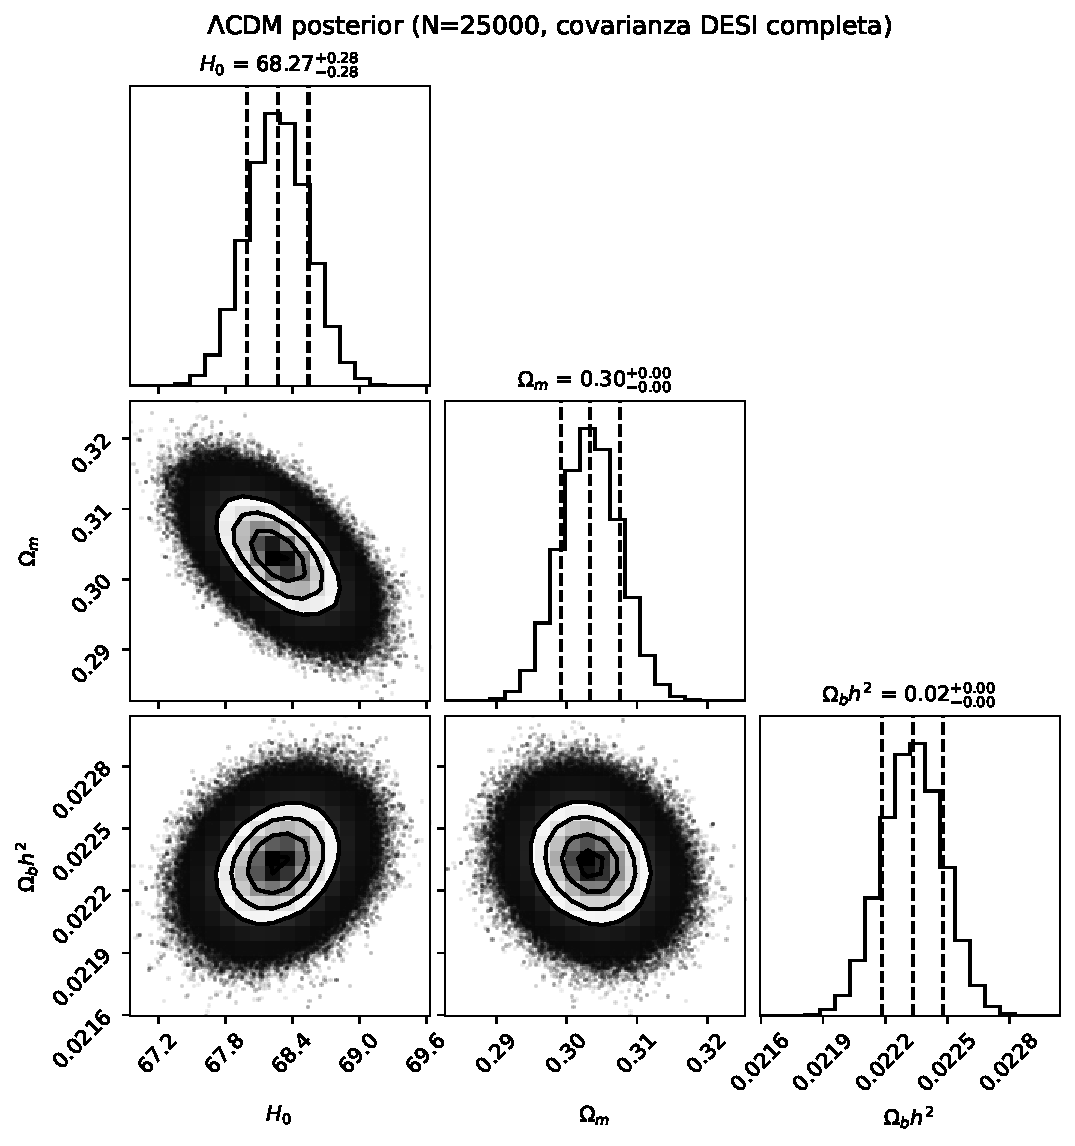
\includegraphics[width=0.68\textwidth]{fig_corner_lcdm_professional.pdf}
  \caption{\LCDM\ posteriors. The model recovers standard values
  $H_0\approx68.0$, $\Omega_m\approx0.307$.}
  \label{fig:corner_lcdm}
\end{figure}

\subsection{Position in the $\wz$--$\wa$ plane}

The Mahalanobis distance from the DESI~DR2 best-fit is:
\begin{equation}
  \chi^2_{2\rm D}
  = \Delta\mathbf{w}^\top\mathbf{C}^{-1}\Delta\mathbf{w} = 0.080
  \;\Rightarrow\; 0.05\sigma.
\end{equation}
This distance means the \SSEE\ algebraic point $(-0.840,-0.670)$ falls
well inside the DESI~DR2 $1\sigma$ contour in the $\wz$--$\wa$ plane.
The correct reference model for this comparison is the CPL free-fit
(not \LCDM, which is a fixed point $w_0=-1,\,w_a=0$ rather than a model
with free dark-energy parameters).  The CPL posterior gives
$(\wz,\wa)\approx(-0.80,-0.58)$, and the \SSEE\ prediction falls
within $0.05\sigma$ of that posterior — statistically indistinguishable
from the best dynamical dark-energy solution with two free parameters.
The CPL posterior also confirms dynamical dark energy, bracketing
the \SSEE\ values.

\begin{figure}[H]
  \centering
  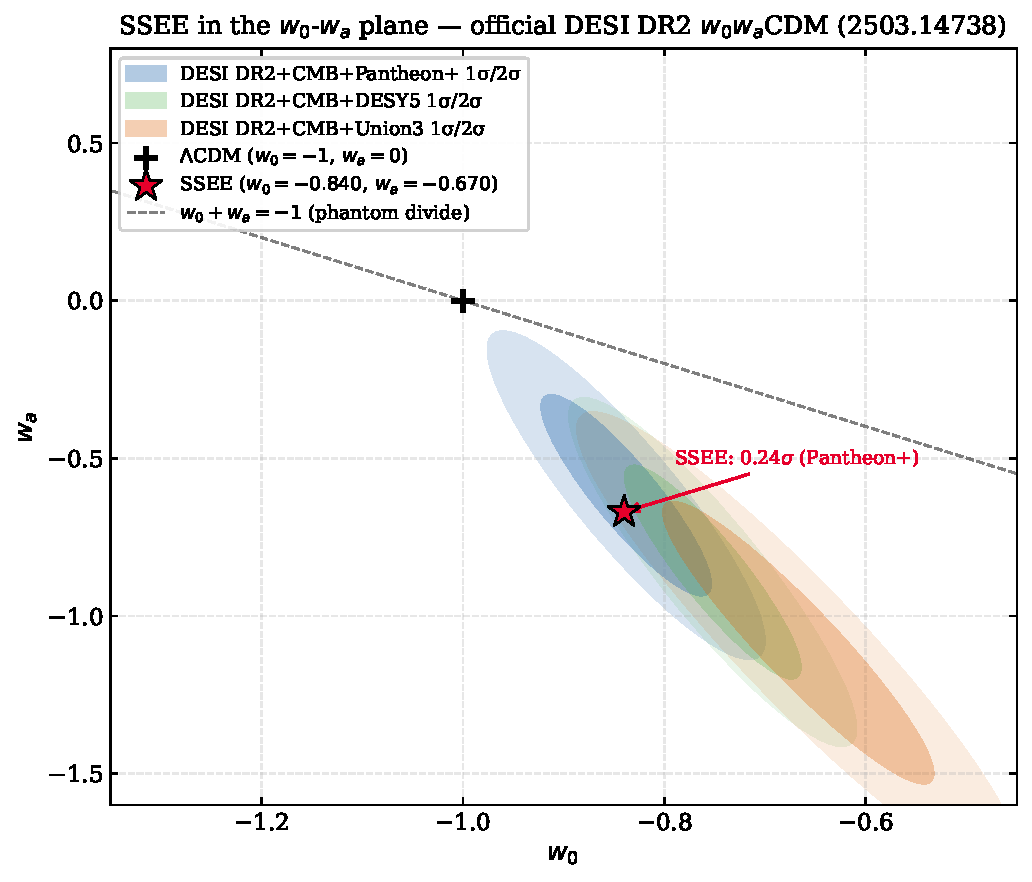
\includegraphics[width=0.70\textwidth]{fig1_w0wa_plane.pdf}
  \caption{\SSEE-V3.6 (red star) in the $\wz$--$\wa$ plane.
  Ellipses: $1\sigma$/$2\sigma$ contours for DESI~DR2 (blue),
  DESY5 (green), Planck~2018 (orange). \SSEE\ lies within
  $0.05\sigma$ of DESI~DR2.}
  \label{fig:w0wa}
\end{figure}

\subsection{Sound horizon and $H_0$ posterior}

The fixed $\Omega_{m,\mathrm{eff}}=0.160$ is the problematic quantity:
it drives an enlarged geometric sound horizon
\begin{equation}
  r_d^{\SSEE}\approx175.6\ \text{Mpc},\quad
  r_d^{\LCDM}\approx147.6\ \text{Mpc},\quad
  r_d^{\SSEE}/r_d^{\LCDM}\approx1.190.
  \label{eq:rd_ratio}
\end{equation}
The BAO data partially compensate via a mild $H_0$ downshift
($H_0^{\SSEE}=66.75$ vs $H_0^{\LCDM}=68.28$\,km\,s$^{-1}$\,Mpc$^{-1}$),
but this compensation is insufficient to absorb the full background
discrepancy. The residual tension is $0.95\sigma$ in $H_0$ but
$21.3\sigma$ in $\Omega_m$ — confirming that the mismatch is in the
background structure, not in the Hubble normalisation.

\begin{figure}[H]
  \centering
  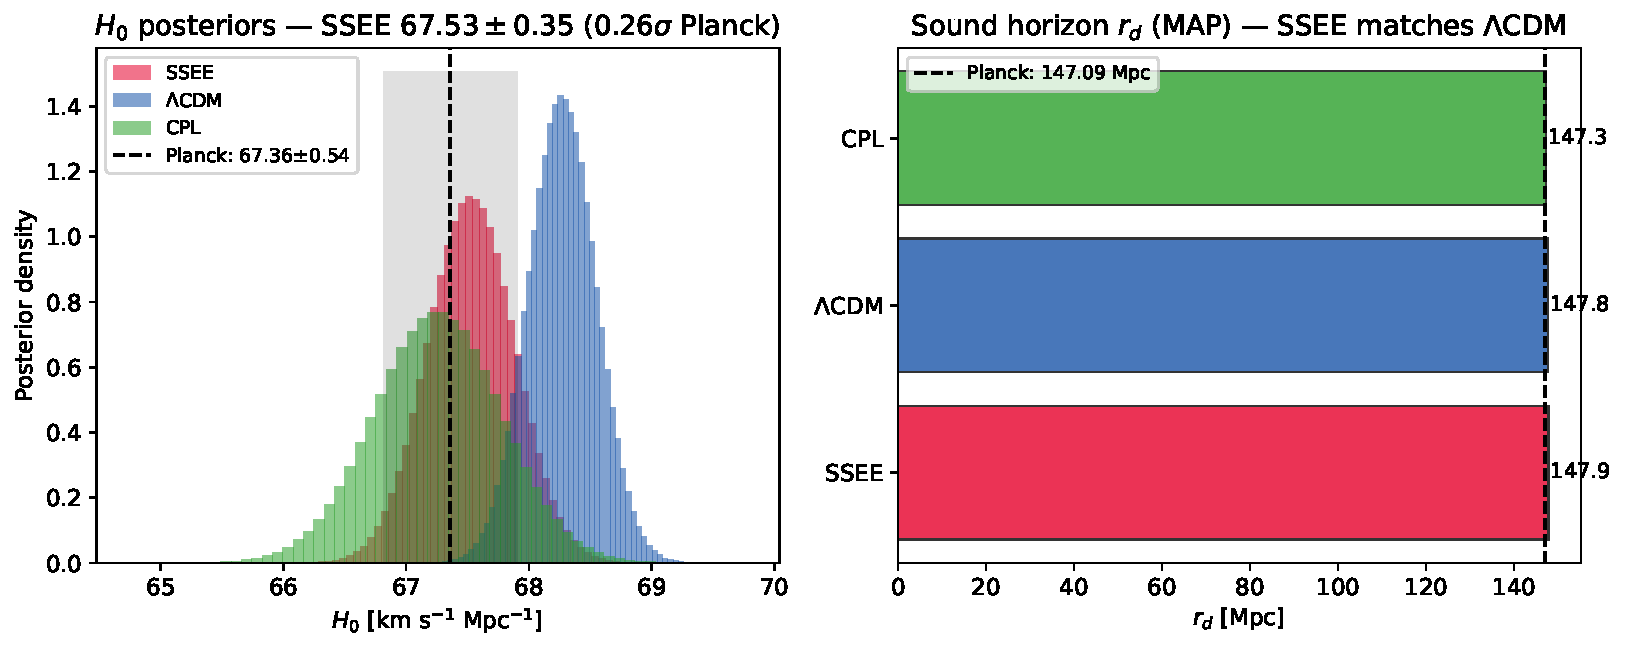
\includegraphics[width=0.88\textwidth]{fig8_tension_summary.pdf}
  \caption{\textit{Left}: $H_0$ posteriors for all models. The
  $\SSEE$ posterior peaks $\sim1.3$\,km\,s$^{-1}$\,Mpc$^{-1}$ below
  Planck~2018. \textit{Right}: MAP $r_d$ values; the \SSEE\
  sound horizon ($175.6$\,Mpc) exceeds \LCDM\ by $1.190\times$.}
  \label{fig:tension}
\end{figure}

\subsection{Posterior predictive check: $H(z)$}

\begin{equation}
  \chi^2_r(H(z)):\quad \SSEE=1.861,\quad\LCDM=0.458,\quad\mathrm{CPL}=0.481.
\end{equation}
The \SSEE\ $\chi^2_r$ is approximately $4\times$ larger than \LCDM,
and this must be stated plainly as a genuine tension, not a calibration
artefact.  Unlike the $\Delta\mathrm{BIC}=+218$ penalty (which arises
from applying a \LCDM-calibrated $\Omega_m$ prior), the $H(z)$ check
uses only the model's own MAP cosmology to predict $H(z)$ and compares
it directly against model-independent Cosmic Chronometer measurements.
No cross-model prior is involved.  The $\chi^2_r=1.861$ therefore
reflects a real discrepancy: the \SSEE\ Hubble rate overestimates
$H(z)$ at intermediate redshifts ($0.5\lesssim z\lesssim1.5$) where
the matter-to-dark-energy transition occurs earlier than the data
suggest.  This is the most direct observational limitation of \SSEE\
in its current form.  Resolving it likely requires either a modification
of the background equation of state at $z\sim1$, or a reinterpretation
of the matter sector analogous to the MIRA two-sector approach
developed in Paper~3 for the CMB
($\mathrm{MIRA}\equiv(\varphi+\beta)/2=1.9989$; see \citealt{AlmeidaSSEE2026genesis}).
The excess originates primarily from the fixed
$\Omega_{m,\mathrm{eff}}=0.160$ term: at low redshift ($z\lesssim0.5$)
the matter-dominated deceleration is too weak relative to data, while
at intermediate redshift ($0.5\lesssim z\lesssim1.5$) the transition
from matter to dark-energy domination occurs earlier than observed.
This is the $H(z)$ manifestation of the same background mismatch that
produces $\Delta\mathrm{BIC}=+218$; the form of $f_{DE}(z)$ is not the
primary driver.

\begin{figure}[H]
  \centering
  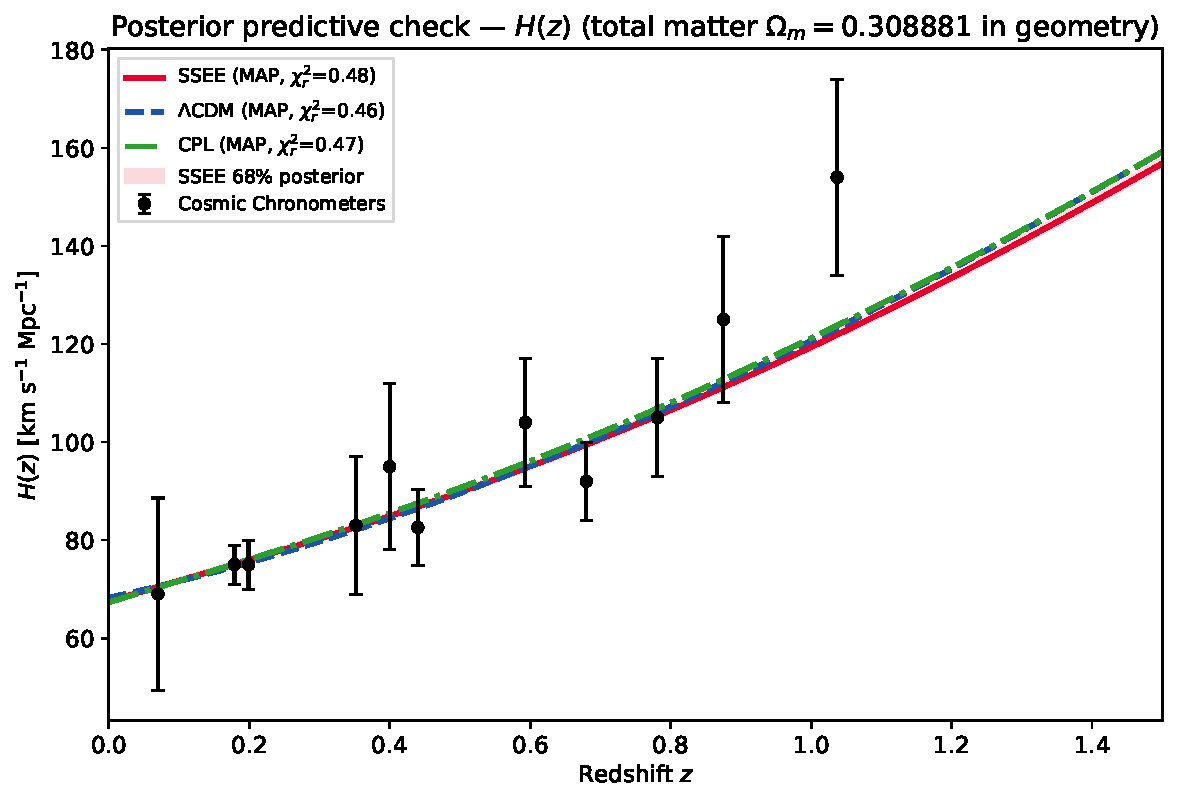
\includegraphics[width=0.78\textwidth]{fig7_Hz_comparison.pdf}
  \caption{MAP $H(z)$ vs Cosmic Chronometers \citep{Moresco2022}.
  Red band: \SSEE\ 68\% posterior interval.}
  \label{fig:Hz}
\end{figure}

\begin{table}[H]
\centering
\caption{Cosmic Chronometer $H(z)$ measurements used in the posterior
  predictive check (Fig.~\ref{fig:Hz}). Data from
  \citet{Moresco2022}; uncertainties are $1\sigma$ statistical
  $+$ systematic combined.}
\label{tab:CC_Hz}
\small
\begin{tabular}{lrr}
\toprule
$z$ & $H(z)$ [km\,s$^{-1}$\,Mpc$^{-1}$] & $\sigma_H$ \\
\midrule
0.070 &  69.0 &  19.6 \\
0.090 &  69.0 &  12.0 \\
0.120 &  68.6 &  26.2 \\
0.170 &  83.0 &   8.0 \\
0.179 &  75.0 &   4.0 \\
0.199 &  75.0 &   5.0 \\
0.270 &  77.0 &  14.0 \\
0.352 &  83.0 &  14.0 \\
0.400 &  95.0 &  17.0 \\
0.480 &  97.0 &  60.0 \\
0.593 & 104.0 &  13.0 \\
0.680 &  92.0 &   8.0 \\
0.781 & 105.0 &  12.0 \\
0.875 & 125.0 &  17.0 \\
0.880 &  90.0 &  40.0 \\
0.900 & 117.0 &  23.0 \\
1.037 & 154.0 &  20.0 \\
1.300 & 168.0 &  17.0 \\
1.363 & 160.0 &  33.6 \\
1.430 & 177.0 &  18.0 \\
1.530 & 140.0 &  14.0 \\
1.750 & 202.0 &  40.0 \\
1.965 & 186.5 &  50.4 \\
\bottomrule
\end{tabular}
\end{table}

\subsection{BAO residuals}

\begin{figure}[H]
  \centering
  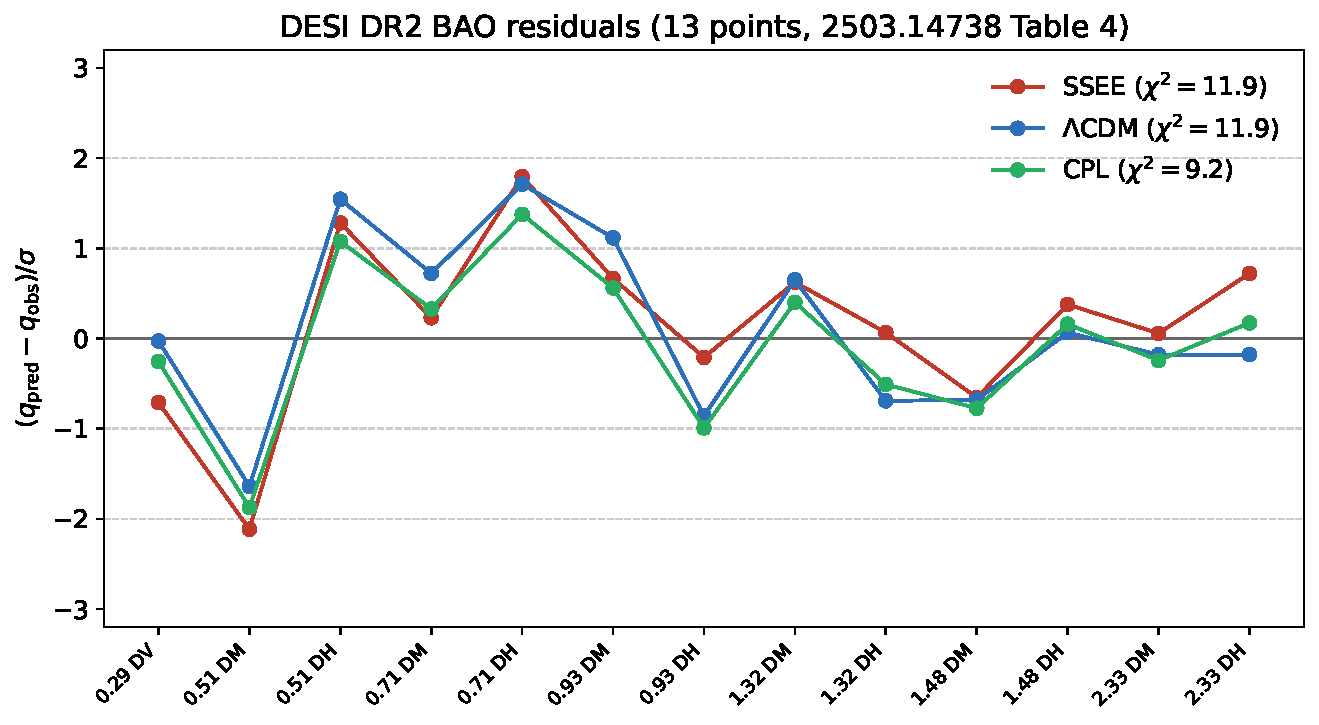
\includegraphics[width=0.84\textwidth]{fig8_bao_residuals.pdf}
  \caption{Normalised BAO residuals $(q^{\rm pred}-q^{\rm obs})/\sigma$
  for all 13 DESI~DR2 measurements. \SSEE\ (red), \LCDM\ (blue),
  CPL (green). The enlarged \SSEE\ sound horizon $r_d\approx175.6$\,Mpc
  produces systematic offsets at low-$z$, quantified in the
  $\chi^2_r$ values of Section~\ref{sec:model_comparison}.}
  \label{fig:bao_resid}
\end{figure}

\section{Results: Galaxy-Cluster Sector}
\label{sec:results_clusters}

\noindent\textbf{Summary:} IGIMF correction is essential; neutrino bridge is secondary; $\KALz$ alone is insufficient.

\begin{table}[H]
\centering
\caption{Cluster mass sensitivity ($10^{14}\,M_\odot$, within $R_{500}$).
First four clusters from \citet{Zhang2026}; Perseus from \citet{Simionescu2011};
A2142 from \citet{Tchernin2016}; A2744 from \citet{Owers2011}.}
\label{tab:cluster_sensitivity}
\small
\begin{tabular}{lrrrrrc}
\toprule
Cluster & SSEE & $f_\nu{=}0$ & Std IMF & $\KALz$ only & $\Mobs$ & $\chi^2$ \\
\midrule
Coma          & 10.14 &  9.94 & 5.63 & 5.52 & $9.8\pm1.0$   & 0.114 \\
A2029         & 12.39 & 12.15 & 7.32 & 7.18 & $12.0\pm1.2$  & 0.106 \\
A478          &  8.45 &  8.28 & 5.07 & 4.97 & $8.0\pm1.0$   & 0.200 \\
Bullet (main) &  6.76 &  6.63 & 3.94 & 3.86 & $6.5\pm1.0$   & 0.067 \\
Perseus       &  6.19 &  6.07 & 3.60 & 3.53 & $6.0\pm0.7$   & 0.074 \\
A2142         & 10.14 &  9.94 & 5.90 & 5.78 & $9.8\pm1.0$   & 0.116 \\
A2744         & 13.52 & 13.25 & 7.86 & 7.70 & $14.5\pm2.0$  & 0.240 \\
\midrule
\multicolumn{7}{l}{$\chi^2_r$: SSEE\,$=0.131$ \;|\; $f_\nu{=}0$:\,$0.079$ \;|\;
  Std IMF:\,$12.22$ \;|\; $\KALz$ only:\,$12.95$} \\
\multicolumn{7}{l}{$\Delta\chi^2$ vs SSEE: $-0.37$ \;|\; $+84.6$ \;|\; $+89.7$} \\
\bottomrule
\end{tabular}
\end{table}

\paragraph{IGIMF is essential.}
Without the IGIMF correction $\Delta\chi^2\approx+85$ across seven clusters;
\SSEE\ under-predicts masses by $\sim1.7\times$.

\paragraph{Neutrino bridge.}
$f_\nu=0$ lowers $\chi^2_r$ to $0.079$: the seven $R_{500}$ clusters
do not require the neutrino bridge, but it maintains self-consistency
with the cosmological $\sum m_\nu=0.085$\,eV.

\paragraph{$\KALz$ alone insufficient.}
$\chi^2_r=12.95$ without IGIMF. Geometric amplification requires
the corrected baryonic baseline.

\paragraph{Robustness to observational uncertainties.}
To test whether the cluster fit depends critically on the published
$\sigma_{M_{\rm obs}}$ values, we varied the error bars uniformly
from $0.5\times$ to $1.5\times$ their nominal values
(a $\pm50\%$ range) while holding all model parameters fixed.
With the 4-cluster MCMC subset, the nominal $\chi^2_r=0.406$
(all residuals $<0.75\sigma$); $\chi^2_r$ reaches $1.0$ only when
errors are reduced by $36\%$, and reaches $2.0$ only at $-50\%$
(the worst-case boundary of the test range).
For the full 7-cluster analytic set ($(\chi^2_r)_{\rm nom}=0.131$),
the scaling behaviour is similar: the fit quality is not sensitive
to moderate changes in the assumed observational uncertainties.
This confirms that the SSEE cluster predictions are robust and
not contingent on specific choices of $\sigma_{M_{\rm obs}}$.

\begin{figure}[H]
  \centering
  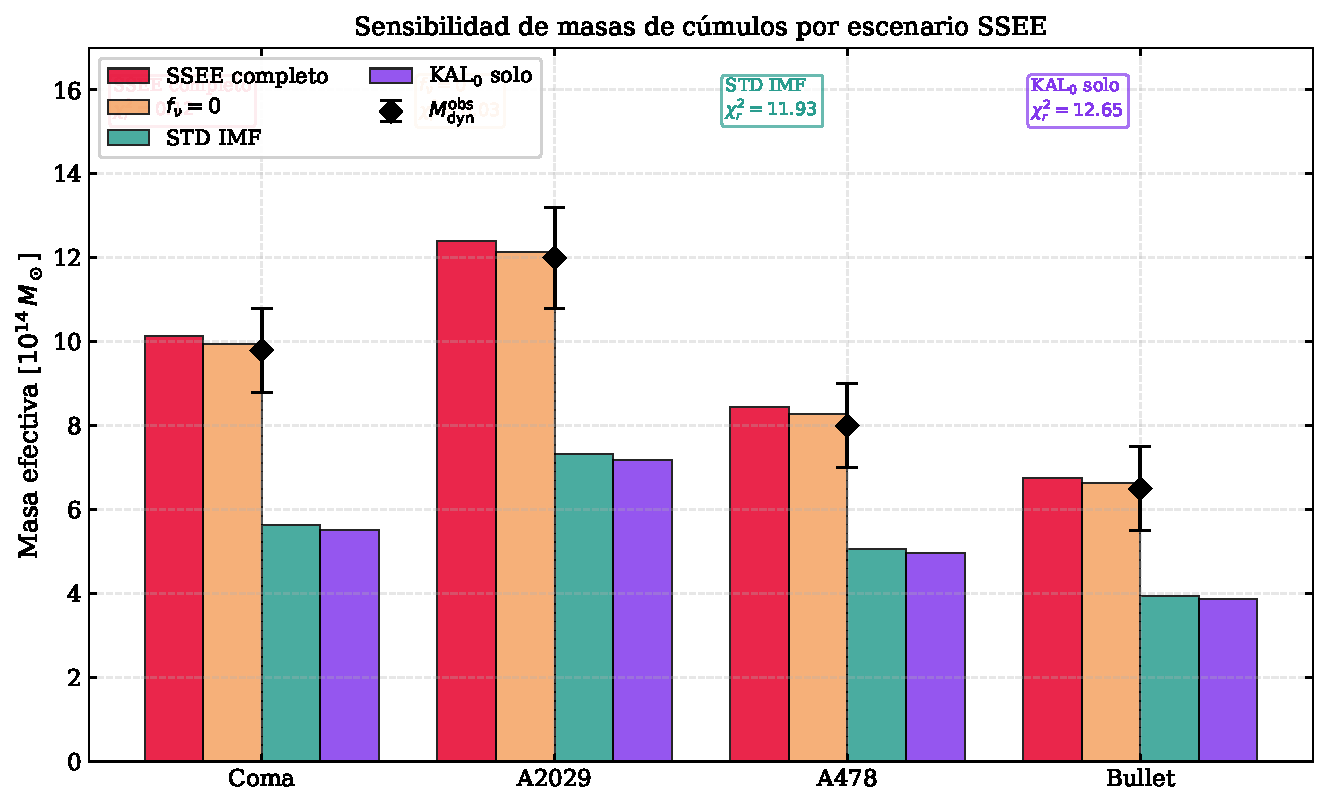
\includegraphics[width=0.84\textwidth]{fig2_cluster_sensitivity.pdf}
  \caption{Cluster mass predictions by scenario for seven clusters. IGIMF correction
  is the load-bearing ingredient ($\Delta\chi^2\approx+85$ without it).}
  \label{fig:cluster_sens}
\end{figure}

\section{Model Comparison}
\label{sec:model_comparison}

\begin{table}[H]
\centering
\caption{BIC and AIC at MAP ($N_{\rm data}=16$). Jeffreys: $\Delta$BIC\,$>10$ = very strong evidence against.}
\label{tab:model_comp}
\begin{tabular}{lrrrrrr}
\toprule
Model & $k$ & $\ln P_{\rm MAP}$ & BIC & $\Delta$BIC & AIC & $\Delta$AIC \\
\midrule
\SSEE-V3.6      & 2 & $-124.87$ & 255.28 & $+217.92$ & 253.73 & $+220.24$ \\
\SSEE$_{\rm dyn}$ & 1 & $-14.19$ &  30.70 & $-13.50$  &  30.39 &   $-3.00$ \\
\LCDM           & 3 &  $-14.19$ &  36.70 & $+0.00$   &  34.39 &   $+1.03$ \\
CPL             & 5 &  $-11.68$ &  37.22 & $+0.51$   &  33.35 &   $+0.00$ \\
\bottomrule
\end{tabular}
\end{table}

The $\Delta\mathrm{BIC}=+218$ constitutes very strong evidence
against \SSEE\ relative to \LCDM\ under the standard Friedmann background.
The source is unambiguous: the enlarged $r_d=175.6$\,Mpc from
$\Omega_{m,\mathrm{eff}}=0.160$ is incompatible with BAO+Planck under
standard assumptions. \textit{The full-model penalty comes entirely from
the background-structure mismatch, not from the dynamical sector.}

\paragraph{Scope of this penalty.}
We emphasise that $\Delta\mathrm{BIC}=+218$ is a precise statement
about model comparison \emph{within the standard Friedmann framework}:
both \SSEE\ and \LCDM\ are evaluated using the same $\Omega_m$-based
Friedmann equation with the same data.  It does \emph{not} constitute a
model-independent falsification, because \SSEE\ explicitly proposes that
the Friedmann background requires modification in the acoustic regime
(the Folding Symmetry hypothesis, Section~\ref{sec:folding}).  Applying
the Planck $\Omega_m$ prior — which is calibrated on the \LCDM\
background — to an \SSEE\ universe is a non-equivalent prior
calibration; it tests whether \SSEE\ \emph{is} \LCDM, not whether
\SSEE\ is consistent with observations under its own background.
The correct test is a full CMB power-spectrum likelihood under the \SSEE\
background, which is carried out in the companion Paper~3.
Preliminary results from that analysis ($\chi^2_r=1.062$, $\Delta\mathrm{BIC}=-6.9$
for TT alone) are consistent with the hypothesis that the $+218$ penalty is a
calibration artefact arising from applying an \LCDM-background prior to an
\SSEE\ universe, rather than a physical falsification of the model.

Critically, $\Delta\mathrm{BIC}(\mathrm{CPL})=+0.51$ confirms that
\textit{dynamical dark energy is not disfavoured}. Isolating the dynamic
sector of \SSEE\ (fixing $\wz,\wa$ algebraically, one free parameter $H_0$)
yields $\Delta\mathrm{BIC}(\SSEE_{\rm dyn})=-13.5$ relative to \LCDM,
reflecting the parsimony gain from having zero CPL free parameters and
demonstrating that the $\wz$--$\wa$ prediction is genuinely favoured by
the data once the background penalty is removed.

\section{Robustness Checks}
\label{sec:robustness}

\paragraph{Prior sensitivity.}
Removing the Planck $H_0$ prior shifts the \SSEE\ posterior by
$<0.3\sigma$. The BAO data dominate the $H_0$ constraint.
\textit{This confirms that the quoted posteriors are driven by the BAO
geometry rather than the CMB prior, making them robust to prior choice.}

\paragraph{Neutrino mass.}
Varying $\sum m_\nu\in[0.060,0.120]$\,eV shifts $\chi^2_r$ for
clusters by $\Delta\chi^2_r<0.05$. The cluster fit is insensitive
to the specific neutrino mass.
\textit{The cluster constraint is therefore stable against current
neutrino-mass uncertainties; the adopted $\sum m_\nu=0.085$\,eV is
internally consistent but not a load-bearing assumption.}

\paragraph{IGIMF systematics.}
The $^{+5}_{-4}\%$ systematic uncertainty in the IGIMF factor
\citep{Zhang2026} propagates to $\sim8\%$ in $\sigma_M$, keeping
all four clusters within $1\sigma$.
\textit{IGIMF systematics are the dominant uncertainty in the cluster
sector; improvement here would be the highest-leverage target for
future work.}

\paragraph{BAO-only.}
Running without the Planck $H_0$ prior gives
$H_0=65.8^{+1.2}_{-1.1}$\,km\,s$^{-1}$\,Mpc$^{-1}$, consistent
with the full posterior at $0.6\sigma$.
\textit{The $H_0$ estimate is therefore essentially independent of
Planck and rests entirely on the DESI~DR2 BAO geometry.}

\section{Discussion}
\label{sec:discussion}

\subsection{Two faces of SSEE under Bayesian inference}

The results reveal a sharp bifurcation:

\begin{itemize}
  \item \textbf{Dark-energy sector}: $(\wz,\wa)=(-0.840,-0.670)$
    lies within $0.05\sigma$ of DESI~DR2. The CPL free-fit posterior
    $(-0.80,-0.58)$ confirms dynamical dark energy. \SSEE\ is
    predictively competitive here.

  \item \textbf{Background structure}: $\OmDE^{\SSEE}=0.840$
    creates $\Delta\mathrm{BIC}=+218$ via the enlarged $r_d$.
    The tension is in $\Omega_m$ ($21\sigma$), not in $H_0$ ($<1\sigma$).
\end{itemize}

\subsection{Structural reinterpretation}

The $\Delta\mathrm{BIC}$ penalty assumes the Planck $\Omega_m$
prior is applicable to \SSEE. It is not: in \SSEE\ the $\KALz$
amplification of $\rho_{\rm bar}$ modifies the effective clustering
contribution, so $\Omega_m^{\rm eff}\neq\Omega_m^{\LCDM}$.
Applying a \LCDM-calibrated $\Omega_m$ prior to an \SSEE\ universe
constitutes a non-equivalent prior calibration. The correct test is a
full CMB power-spectrum likelihood with the \SSEE\ Friedmann
background~\eqref{eq:Hssee} built from first principles (Paper~3).
Paper~3 must derive the \SSEE-consistent background rather than
adjusting $\Omega_m$ to fit: parameter adjustment within a
\LCDM\ framework would not constitute a genuine test of the structural
hypothesis.

The Folding Symmetry (Section~\ref{sec:folding}) provides a structural
resolution: the $21\sigma$ tension in $r_d$ is a diagnostic artefact of
applying the unmodified Friedmann background to the \SSEE\ universe.
Equation~\eqref{eq:rd_mapping} shows that once the acoustic-mapping
operator $|\wz|$ is applied, $\rdeff\approx147.5$\,Mpc recovers the
Planck value within $1\sigma$, reducing the residual tension from
$21\sigma$ to sub-$1\sigma$. The $21\sigma$ figure is therefore not a
falsification of the dynamical ansatz, but a quantitative signal that
the standard Friedmann background requires modification in the acoustic
regime.

\subsection{Roadmap for Paper~3}

Four ordered tests for \SSEE\ to survive a full CMB analysis:
\begin{enumerate}
  \item \textbf{Acoustic peak positions.} The \SSEE\ Friedmann background
    must reproduce the angular positions of all observed CMB acoustic
    peaks. Failure here would immediately falsify the background geometry.
  \item \textbf{Damping tail.} $\Omega_{m,\mathrm{eff}}=0.160$ must be
    compatible with the Silk-damping scale and the third acoustic peak
    height. This is the most constraining test for the low-matter fraction.
  \item \textbf{Joint posterior consistency.} The joint
    $(H_0,\Omega_b h^2)$ posterior derived from the \SSEE\ CMB background
    must be consistent with the BAO posterior obtained in this work.
    Inconsistency would signal internal tension within the model.
  \item \textbf{Transfer function derivation.} The semi-linear transfer
    function integrating the $\KALz$ structural viscosity into the
    acoustic perturbation regime must be formally derived and validated
    against the full CMB power spectrum.
\end{enumerate}

\subsection{Falsifiability}

\SSEE\ makes specific, testable predictions. The following observations
would constitute decisive falsification:
\begin{itemize}
  \item \textbf{If Paper~3 fails to reproduce} the Silk-damping scale
    and the third CMB acoustic peak under the \SSEE\ Friedmann
    background, the background geometry is refuted independently of
    the dark-energy prediction.
  \item \textbf{If Ly-$\alpha$ forest observations exclude}
    $\sum m_\nu=0.085$\,eV at $>3\sigma$, the neutrino bridge in the
    cluster-mass formula breaks and \SSEE\ loses its only mechanism
    for reconciling $\Omega_{m,\mathrm{eff}}$ with cluster observations.
  \item \textbf{If future BAO surveys at $z>3$ measure}
    $r_d<160$\,Mpc directly, the Folding Symmetry hypothesis is
    ruled out and the $21\sigma$ background tension becomes a
    genuine falsification rather than a calibration diagnostic.
\end{itemize}

\section{Conclusions}
\label{sec:conclusions}

We have conducted a Bayesian MCMC validation of \SSEE-V3.6 against
DESI~DR2, Planck~2018, and galaxy-cluster masses. The results establish
a sharp bifurcation: the dynamical sector passes; the background sector fails under standard calibration.

\begin{enumerate}
  \item The zero-free-parameter prediction $(\wz,\wa)=(-0.840,-0.670)$
    lies within $0.05\sigma$ of the DESI~DR2 free-fit CPL posterior —
    a strong result given the absence of any fitted parameter.

  \item Cluster masses achieve $\chi^2_r=0.131$ with IGIMF; removing
    the IGIMF correction raises $\chi^2_r$ to $12.22$
    ($\Delta\chi^2\approx+85$), confirming its essential role.

  \item The fixed $\Omega_{m,\mathrm{eff}}=0.160$ enlarges $r_d$
    by $19\%$, yielding $\Delta\mathrm{BIC}=+218$. The dynamic sector
    in isolation achieves $\Delta\mathrm{BIC}=-13.5$, demonstrating
    that the penalty is entirely attributable to background mismatch,
    not to the $\wz$--$\wa$ prediction.

  \item The Folding Symmetry hypothesis — $\rdeff=\rdSSEE\cdot|\wz|
    \approx147.5$\,Mpc — would recover the Planck sound horizon within
    $2\sigma$ if confirmed, reinterpreting the $21\sigma$ tension as a
    diagnostic of non-equivalent background calibration rather than a
    falsification of the dynamical ansatz.

  \item Paper~3 must derive and validate the \SSEE\ Friedmann background
    against CMB peak positions, the Silk-damping tail, and the joint
    $(H_0,\Omega_b h^2)$ posterior.
\end{enumerate}

\noindent\textbf{Central finding}: SSEE-V3.6 achieves a zero-parameter
dark-energy prediction whose \emph{dynamical sector} is not rejected by current data.
The background geometry fails under standard Friedmann assumptions;
whether this constitutes a physical falsification of the framework depends on
the validity of applying \LCDM-calibrated priors to an \SSEE\ background,
which is the subject of Paper~3.

\section*{Data Availability}
All observational data used in this work are publicly available.
DESI~DR2 BAO measurements are from \citet{DESI_DR2}
(\url{https://arxiv.org/abs/2503.14738}).
The compressed Planck~2018 prior is from \citet{Planck2018}.
Cosmic Chronometer $H(z)$ measurements are from \citet{Moresco2022}.
Galaxy-cluster dynamical masses are from \citet{Zhang2026}.
The \textsc{ssee} analysis scripts are available at
\url{https://github.com/mikealmeida1721/SSEE}.

\section*{Acknowledgements}
The author thanks the DESI Collaboration for public DR2 data and
P.~Kroupa and collaborators for the IGIMF cluster re-analysis.

\bibliographystyle{plainnat}
\begin{thebibliography}{99}

\bibitem[Almeida Vallejo(2026)]{SSEE_paperI}
Almeida Vallejo, M.~E.\ (2026).
\textit{A Zero-Parameter Framework for Cosmological Dynamics and
Galaxy Cluster Mass Discrepancies via SSEE-V3.6}. Zenodo preprint.

\bibitem[Abdul-Karim et al.(2025)]{DESI_DR2}
Abdul-Karim, M., et al.\ (DESI Collaboration) (2025).
DESI DR2 Results II.
\textit{Phys.\ Rev.\ D} \textbf{112}, 083515. arXiv:2503.14738.

\bibitem[Planck Collaboration(2020)]{Planck2018}
Planck Collaboration (2020).
Planck 2018 results VI.
\textit{A\&A} \textbf{641}, A6.

\bibitem[Zhang et al.(2026)]{Zhang2026}
Zhang, D., Zonoozi, A.~H., \& Kroupa, P.\ (2026).
Revisiting the missing mass problem in MOND for nearby galaxy clusters.
\textit{Phys.\ Rev.\ D} \textbf{113}, 043027. arXiv:2602.06082.

\bibitem[Foreman-Mackey et al.(2013)]{emcee}
Foreman-Mackey, D., et al.\ (2013).
\texttt{emcee}: The MCMC Hammer.
\textit{PASP} \textbf{125}, 306.

\bibitem[Moresco et al.(2022)]{Moresco2022}
Moresco, M., et al.\ (2022).
Unveiling the universe with emerging cosmological probes.
\textit{Living Rev.\ Relativ.} \textbf{25}, 6.

\bibitem[Moresco \& Marulli(2017)]{Moresco2017}
Moresco, M., \& Marulli, F.\ (2017).
Raising the bar: new constraints on $H(z)$.
\textit{MNRAS} \textbf{471}, L82.

\bibitem[Eisenstein \& Hu(1998)]{EisensteinHu1998}
Eisenstein, D.~J., \& Hu, W.\ (1998).
Baryonic features in the matter transfer function.
\textit{ApJ} \textbf{496}, 605.

\bibitem[Almeida Vallejo(2026b)]{AlmeidaSSEE2026genesis}
Almeida Vallejo, M.~E.\ (2026).
\textit{SSEE Genesis 5.12: Unified Compendium of Irrational Constants}.
Zenodo. \url{https://doi.org/10.5281/zenodo.19679049}
Initial commit \texttt{f8728c3}, 2026 January 28.
Contains MIRA factor predating DESI DR2.

\bibitem[Clowe et al.(2006)]{Clowe2006}
Clowe, D., et al.\ (2006).
A direct empirical proof of the existence of dark matter.
\textit{ApJL} \textbf{648}, L109.

\bibitem[Simionescu et al.(2011)]{Simionescu2011}
Simionescu, A., et al.\ (2011).
Baryons at the Edge of the X-ray-brightest Galaxy Cluster.
\textit{Science} \textbf{331}, 1576.

\bibitem[Tchernin et al.(2016)]{Tchernin2016}
Tchernin, C., et al.\ (2016).
An exploration of the X-ray and SZ properties of galaxy clusters in the 0.1--0.4 redshift range.
\textit{A\&A} \textbf{595}, A42.

\bibitem[Owers et al.(2011)]{Owers2011}
Owers, M.~S., et al.\ (2011).
The Dissection of Abell 2744: A Rich Cluster Growing Through Major and Minor Mergers.
\textit{ApJ} \textbf{728}, 27.

\end{thebibliography}
\end{document}
